\documentclass{beamer}

\usepackage[utf8]{inputenc}
\usepackage{minted}
\usepackage{listings}
\usepackage{graphicx}
\usepackage{xcolor}


%\usetheme{metropolis}
%\usecolortheme{beaver}
\usetheme{Madrid}
\useinnertheme{circles}
\definecolor{ssgreen}{HTML}{669B41}
\usecolortheme[named=ssgreen]{structure}
\setbeamertemplate{navigation symbols}{}

\AtBeginEnvironment{frame}{\setcounter{footnote}{0}}

\title[Kubernetes]{Introduction to Kubernetes}
\author{Ed MacDonald}
\institute{Solution Street}
\date{July 2020}

\begin{document}
\frame{\titlepage}

\begin{frame}
\frametitle{What is Kubernetes?}
A Container Orchestration Framework
\end{frame}

\begin{frame}
\frametitle{Kubernetes API}
Most Kubernetes API calls involve either:
\begin{itemize}
    \item You telling Kubernetes what you want the state of a given set of objects to converge to, or
    \item You asking Kubernetes what the current state of a given set of objects is
\end{itemize}
\end{frame}

\begin{frame}
\frametitle{Kubernetes API}
Think of the Kubernetes API as a way to:
\begin{itemize}
    \item Send YAML documents to Kubernetes which specify components you would like to create in your cluster.
    \item Send requests to Kubernetes that specify updates components in your cluster.
    \item Sent requests asking Kubernetes for the current state of components in your cluster.
\end{itemize}
\end{frame}

\begin{frame}
    \begin{center}
        \Huge Tools
    \end{center}
\end{frame}

\begin{frame}
    \frametitle{minikube\footnotemark}
    \begin{itemize}
        \item Easiest way to install a cluster on your machine.
        \item For development purposes only!
    \end{itemize}
    \footnotetext[1]{https://kubernetes.io/docs/tasks/tools/install-minikube/}
\end{frame}

\begin{frame}
\frametitle{kubectl\footnotemark}
\begin{itemize}
\item kubectl is a command line tool used to communicate with Kubernetes clusters.
\item It provides a convenient way to speak with Kubernetes via its API.
\item We will be using it to update components in our cluster and view their state.
\item You \textbf{\textit{can}} use it to create components, but there is a better way to do that...
\end{itemize}
\footnotetext[1]{https://kubernetes.io/docs/tasks/tools/install-kubectl/}
\end{frame}

\begin{frame}
\frametitle{helm\footnotemark}
\begin{itemize}
    \item helm is a tool for packaging and deploying Kubernetes apps.
    \item For our purposes, just think of as a way to package all the YAML files that create the components that make your app, and then deploy them to a cluster.
\end{itemize}
\footnotetext[1]{\href{https://helm.sh/}{https://helm.sh/}}
\end{frame}

\begin{frame}
    \begin{center}
        \Huge Kubernetes Architecture Overview With Sample Apps
    \end{center}
\end{frame}

\begin{frame}
\frametitle{Kubernetes Nodes}
\begin{itemize}
\item Kubernetes Nodes are compute instances (e.g.: virtual machines, bare metal servers) running the Kubernetes software components that allow them to communicate and cooperate with each other to run your application(s)
\item Kubernetes schedules Pods to run on the nodes that make up the cluster.
\end{itemize}
\end{frame}

% https://www.patrickbaylis.com/posts/2018-10-11-beamer-resizing/
\begin{frame}
    \frametitle{Kubernetes Nodes}
    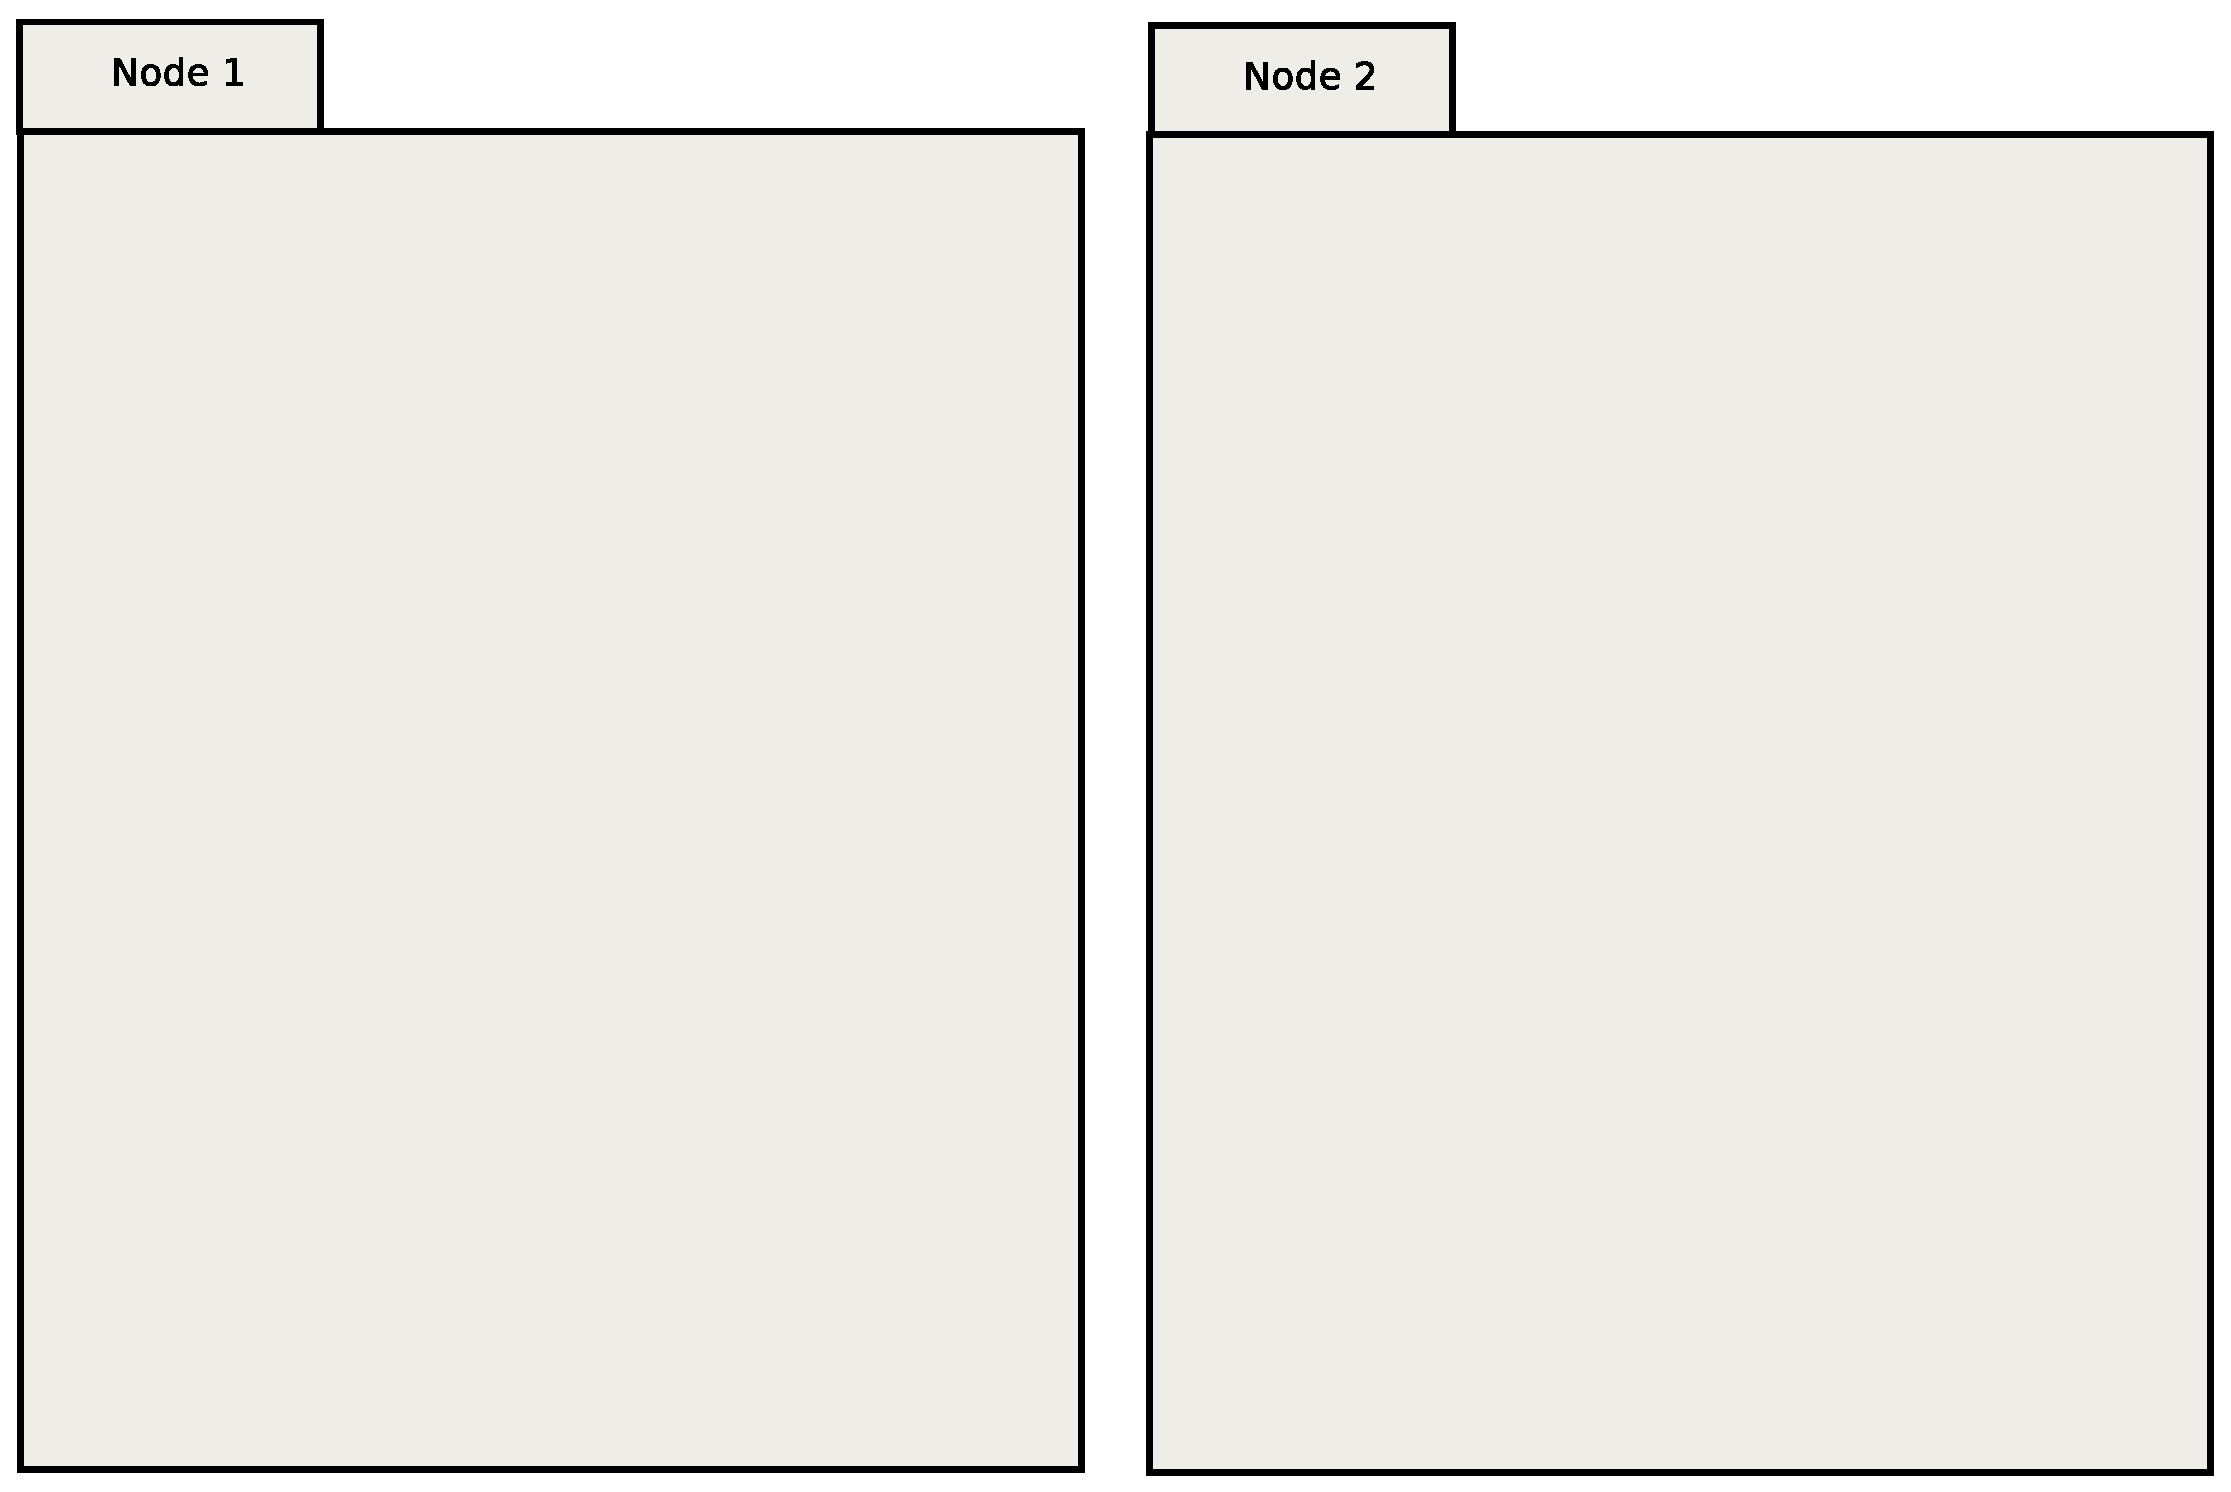
\includegraphics[width=\textwidth,height=0.85\textheight,keepaspectratio]{graphics/00-nodes.eps}
\end{frame}

\begin{frame}
\frametitle{Pods}
Pods (not containers!) are the fundamental building blocks of a Kubernetes application
\begin{itemize}
    \item A Pod is a group of one or more containers that work closely together on a specific task.
    \item Containers in a Pod can access the same volumes.
    \item Some Containers in a Pod can be Init Containers. They run before other pods start and are used to perform initialization tasks. The can communicate with other pods through the aforementioned shared volumes.
\end{itemize}
\end{frame}

\begin{frame}
    \frametitle{System Pods}
    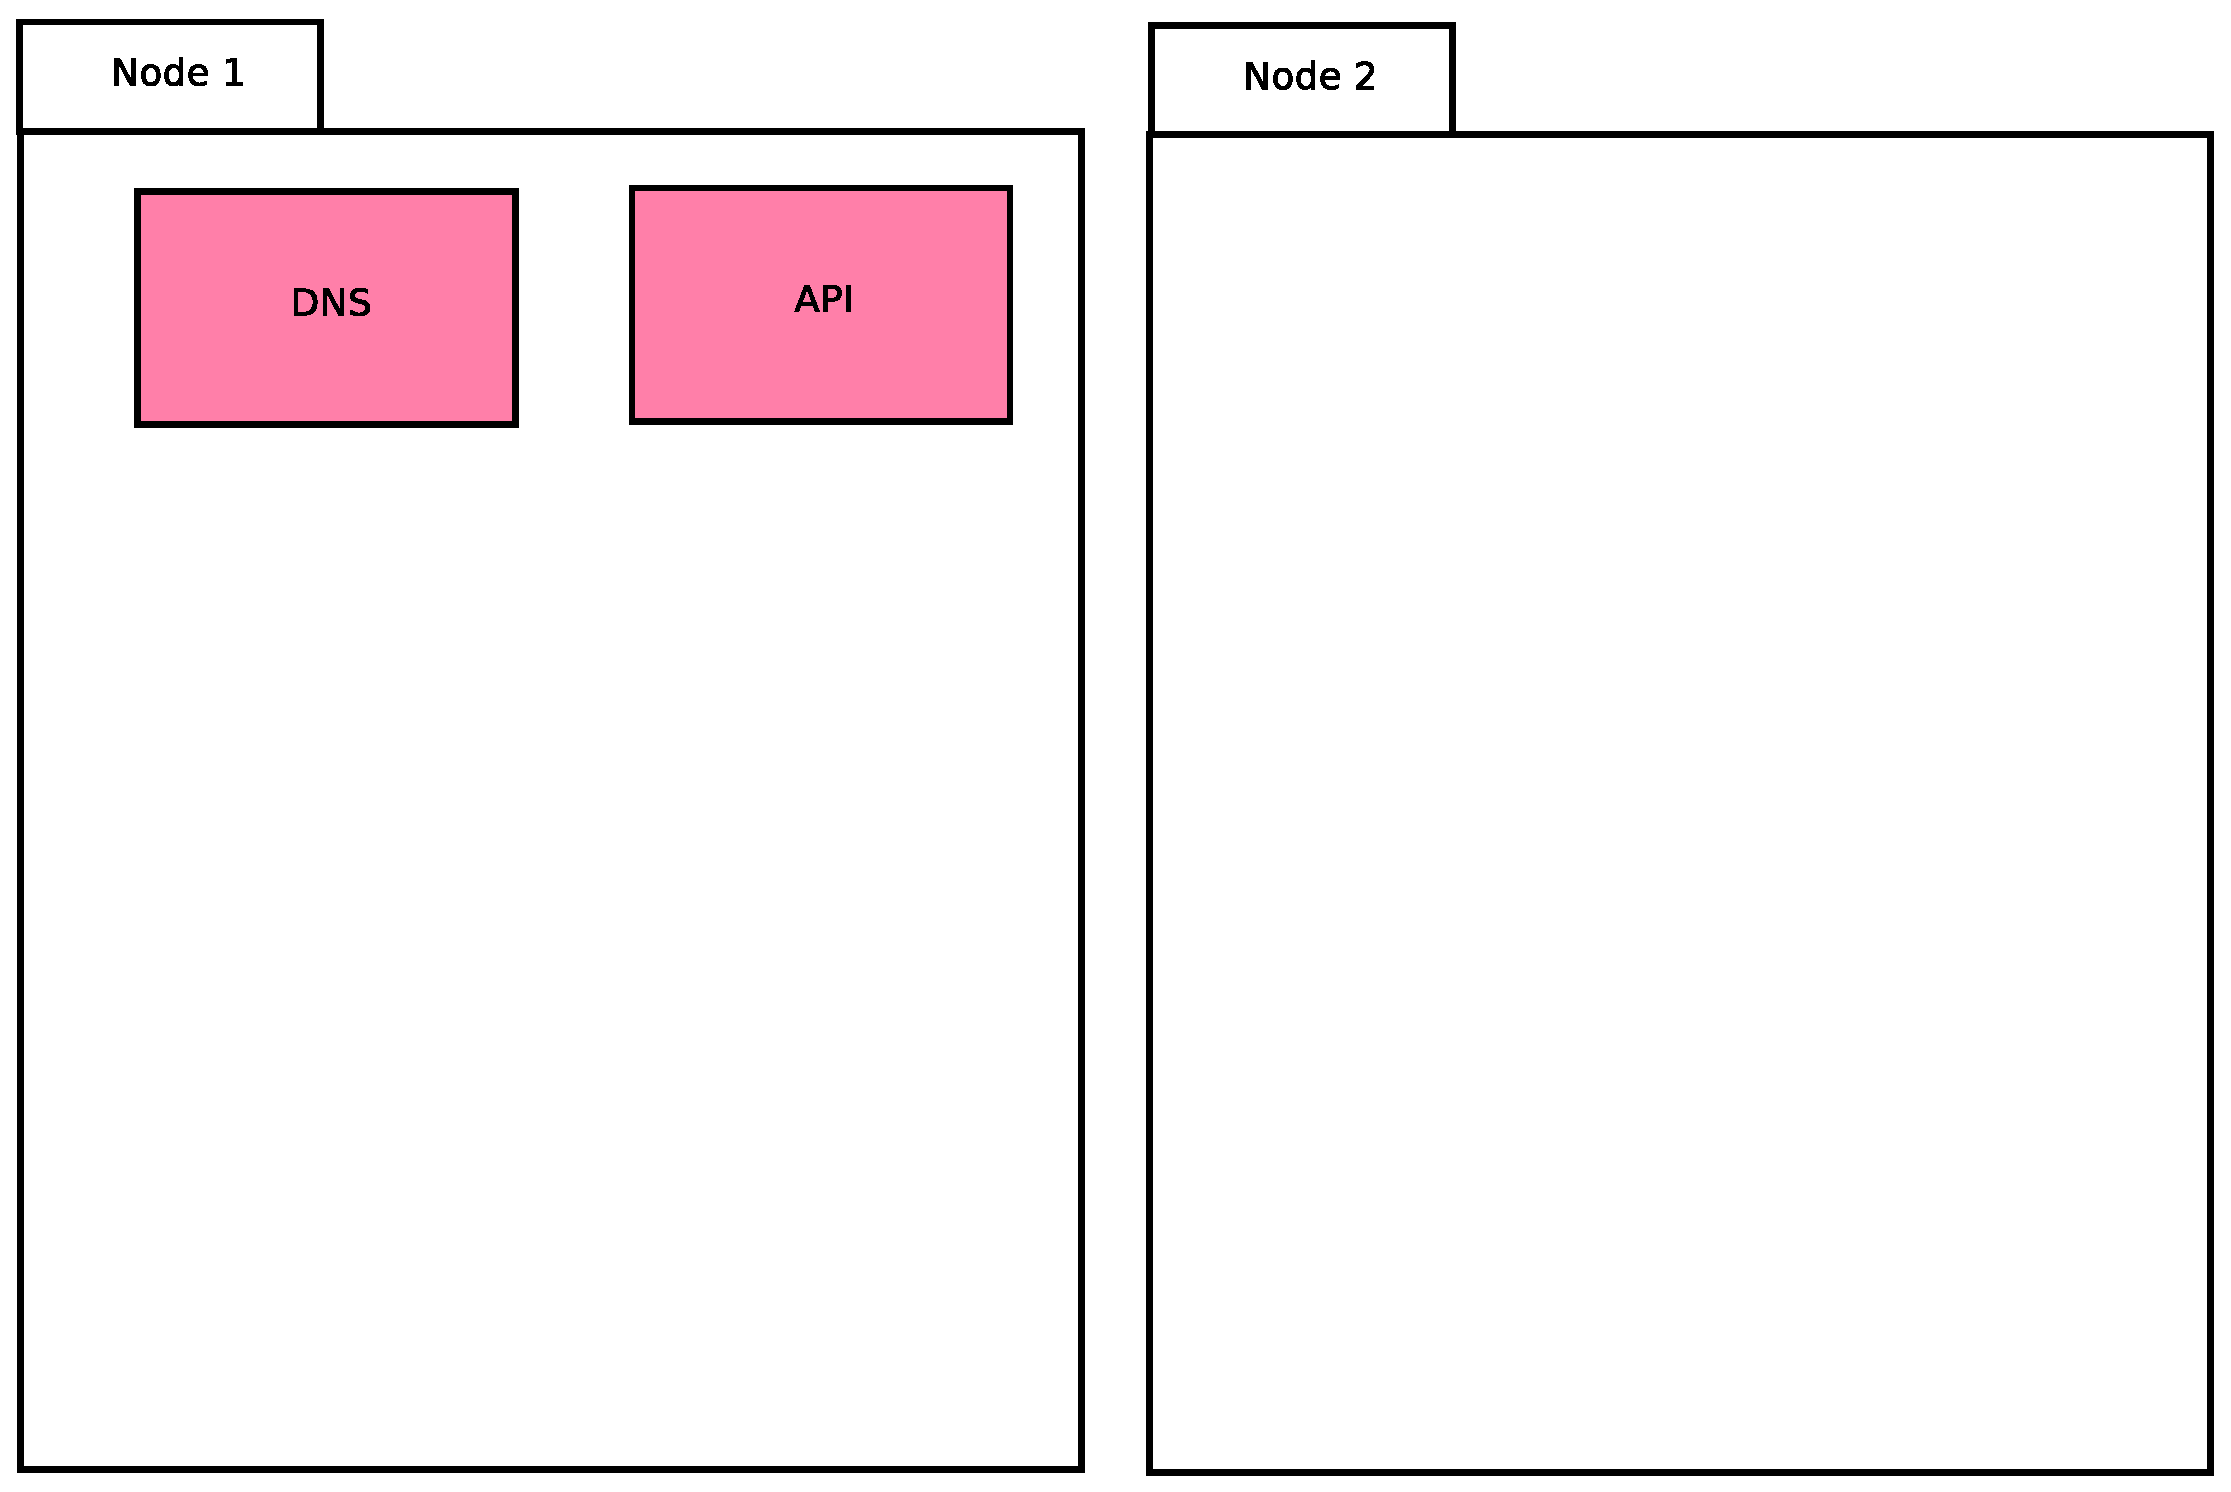
\includegraphics[width=\textwidth,height=0.85\textheight,keepaspectratio]{graphics/01-systemPods.eps}
\end{frame}

\begin{frame}
\frametitle{The Sample Apps}
I wrote two apps that do nothing other than suggest a random Subreddit.
\begin{itemize}
    \item One is stateless and selects at random from a list of 280 Subreddits.
    \item The other is stateful and removes each Subreddit from the list upon suggesting it.
\end{itemize}
\end{frame}

\begin{frame}
    \frametitle{Stateless Application Pods}
    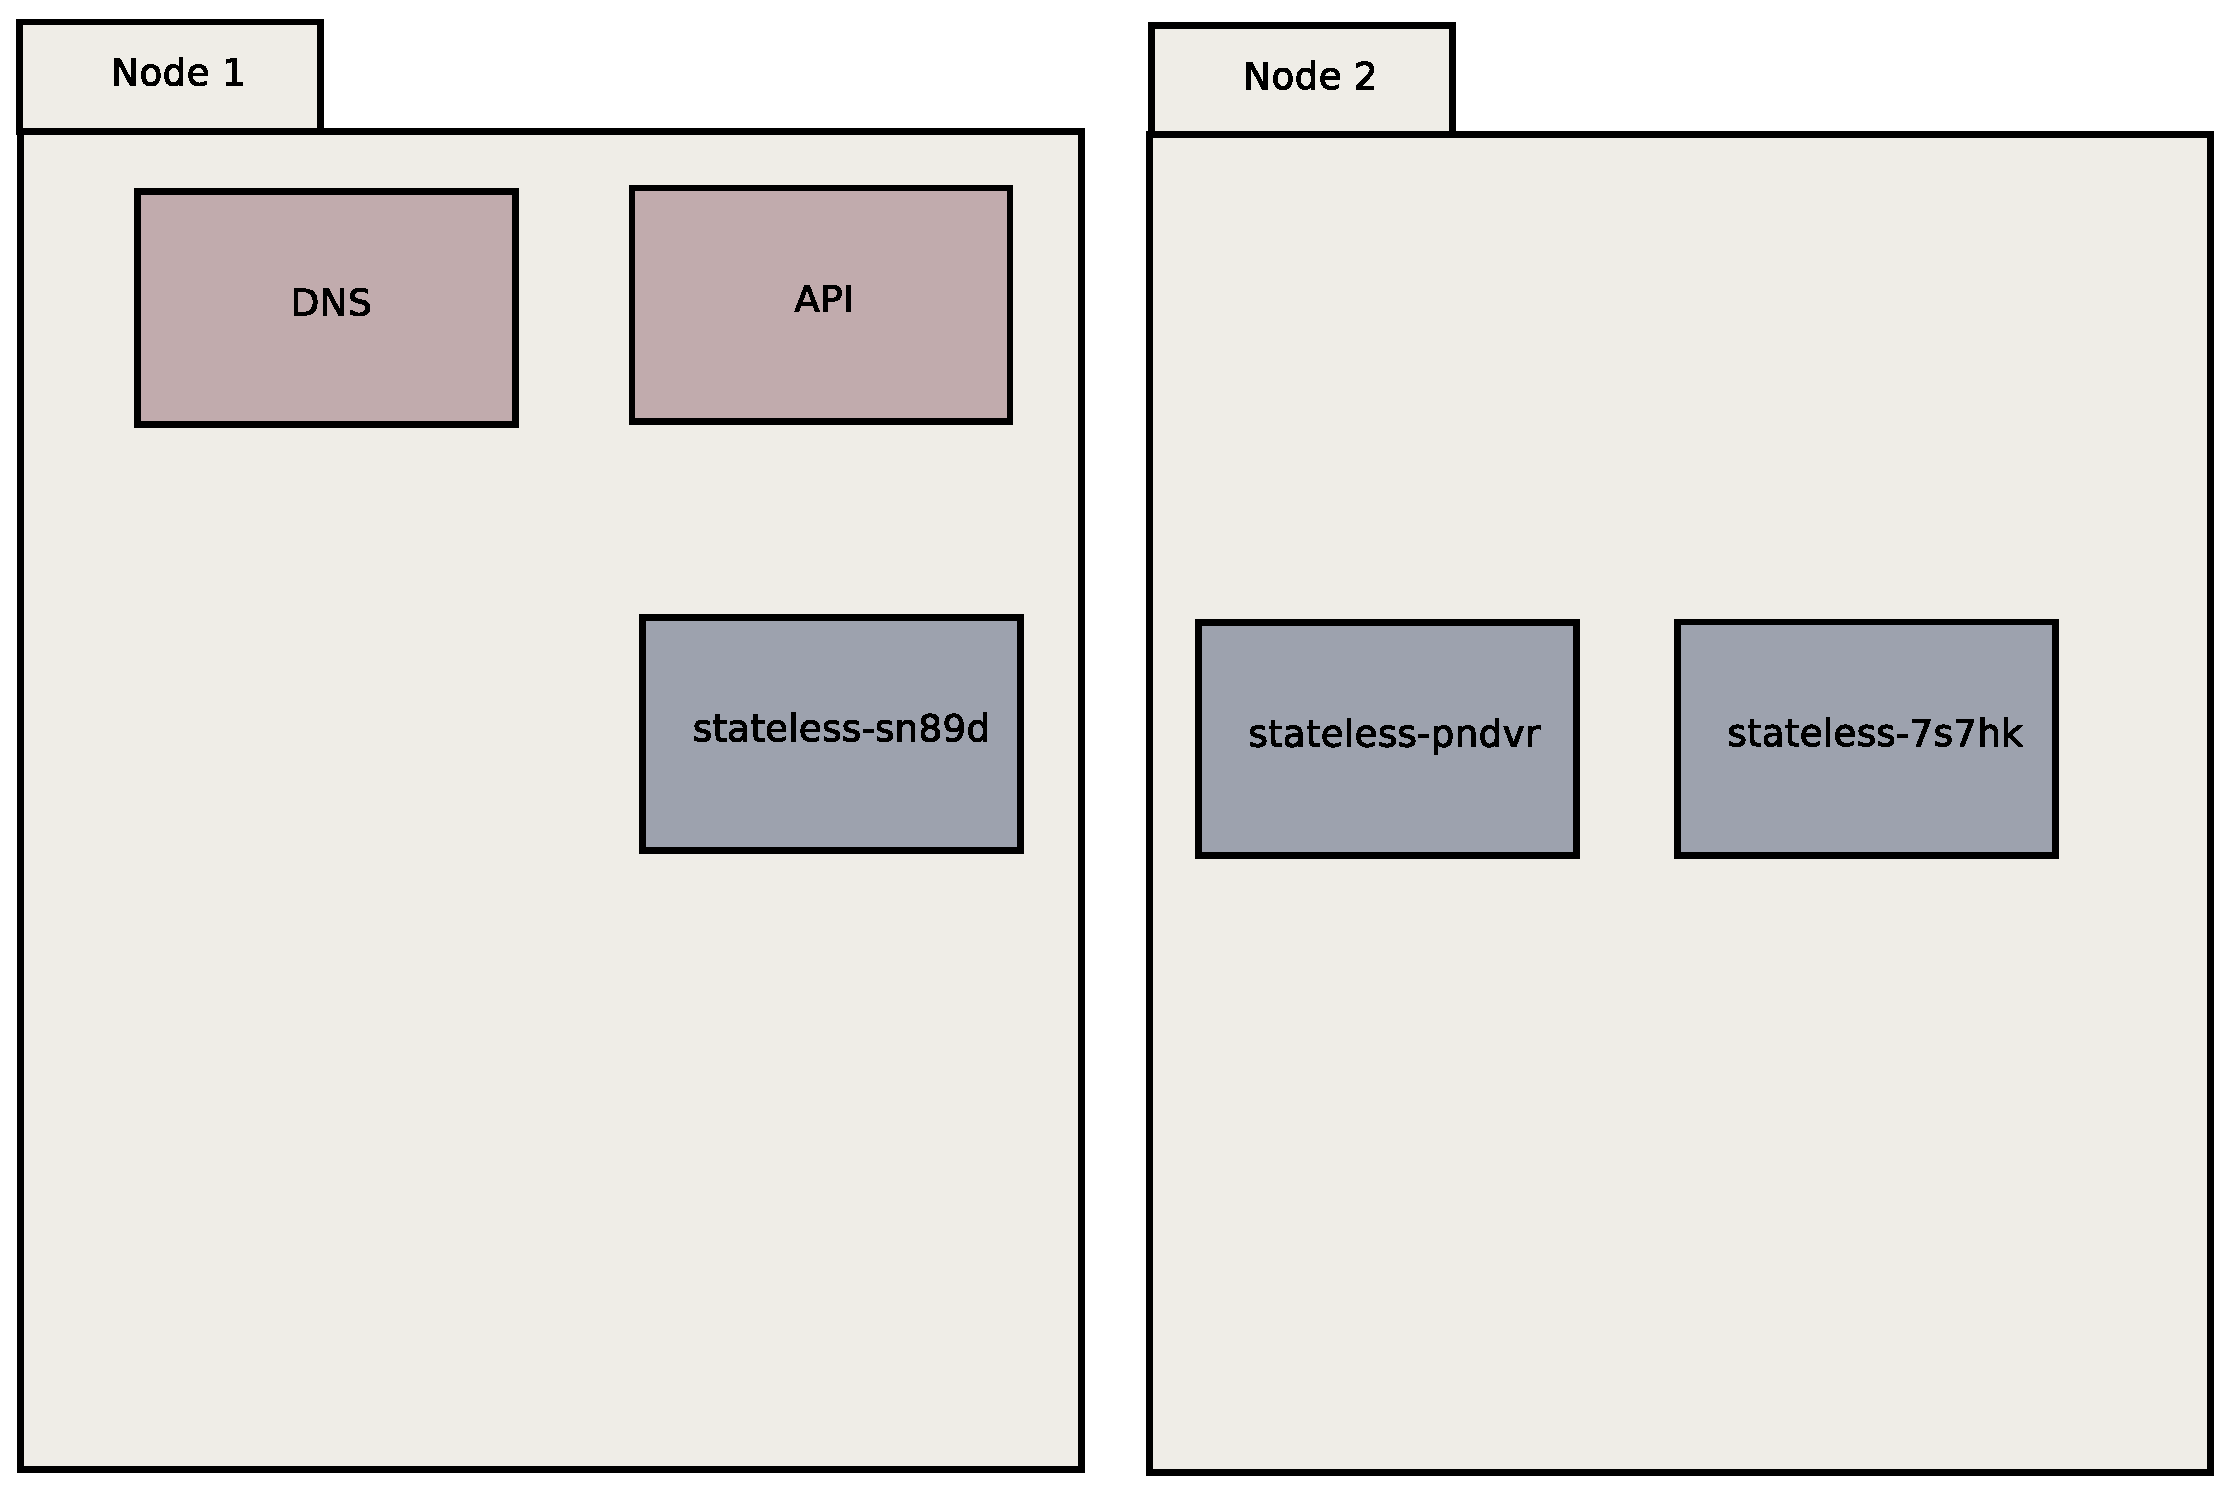
\includegraphics[width=\textwidth,height=0.85\textheight,keepaspectratio]{graphics/02-statelessAppPods.eps}
\end{frame}

\begin{frame}
    \frametitle{Stateful Application Pods}
    \includegraphics[width=\textwidth,height=0.85\textheight,keepaspectratio]{graphics/03-statefulAppPods.eps}
\end{frame}

\begin{frame}
\frametitle{ReplicaSets}
\begin{itemize}    
    \item ReplicaSets allow you to declare to Kubernetes how many of a given type of Pod you wish to have running.
    \item Pods in a ReplicaSet are treated as if they are Stateless.
\end{itemize}
\end{frame}

\begin{frame}
    \frametitle{Deployments}
    \begin{itemize}
        \item Deployments are an even higher level abstraction than Replica Sets.
        \item The docs say they provide "declarative updates to Pods".
        \item I'll use them in my example instead of Replica Sets, but we won't use any of their additional features.
    \end{itemize}
\end{frame}

\begin{frame}
    \frametitle{Deployment}
    \includegraphics[width=\textwidth,height=0.85\textheight,keepaspectratio]{graphics/04-deployment.eps}
\end{frame}

\begin{frame}
    \frametitle{Stateful Sets}
    StatefulSets add features needed by stateful apps, namely:
    \begin{itemize}
        \item Pods in a StatefulSet each have a persistent network identity.
        \item Pods in a StatefulSet each have persistent storage.
    \end{itemize}
\end{frame}

\begin{frame}
    \frametitle{Statefulset}
    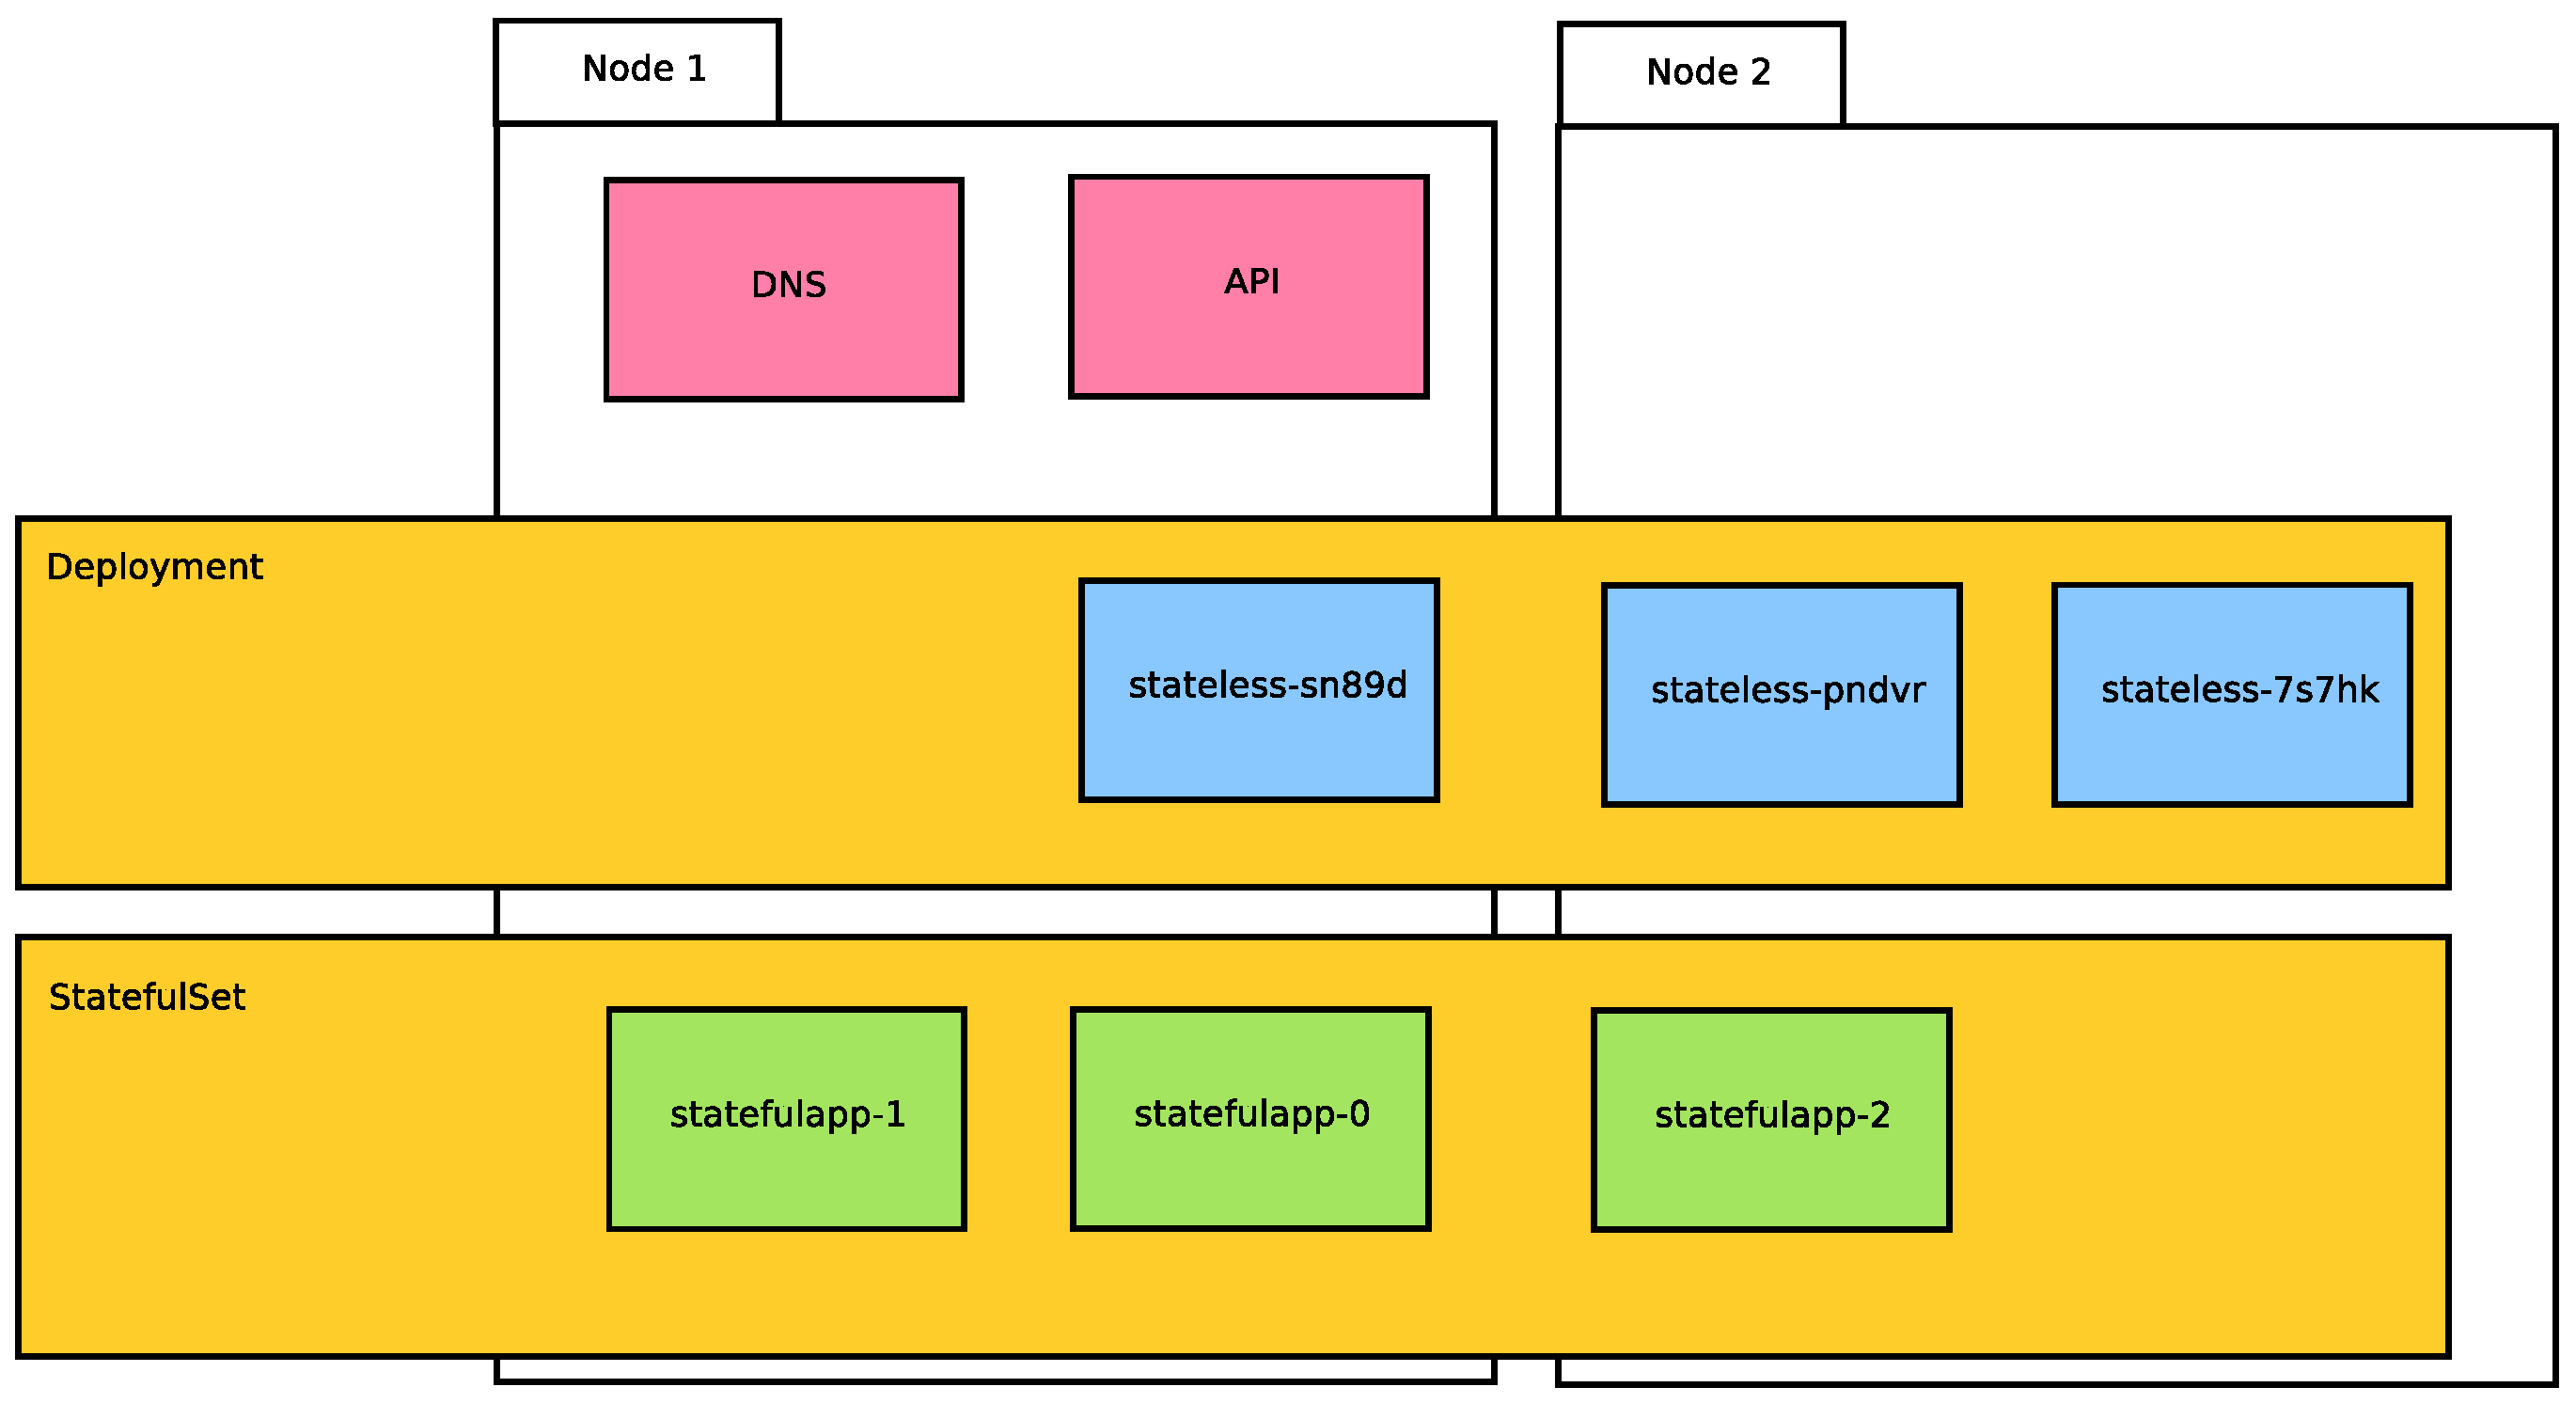
\includegraphics[width=\textwidth,height=0.85\textheight,keepaspectratio]{graphics/05-statefulSet.eps}
\end{frame}

\begin{frame}
    \frametitle{Persistent Storage}
    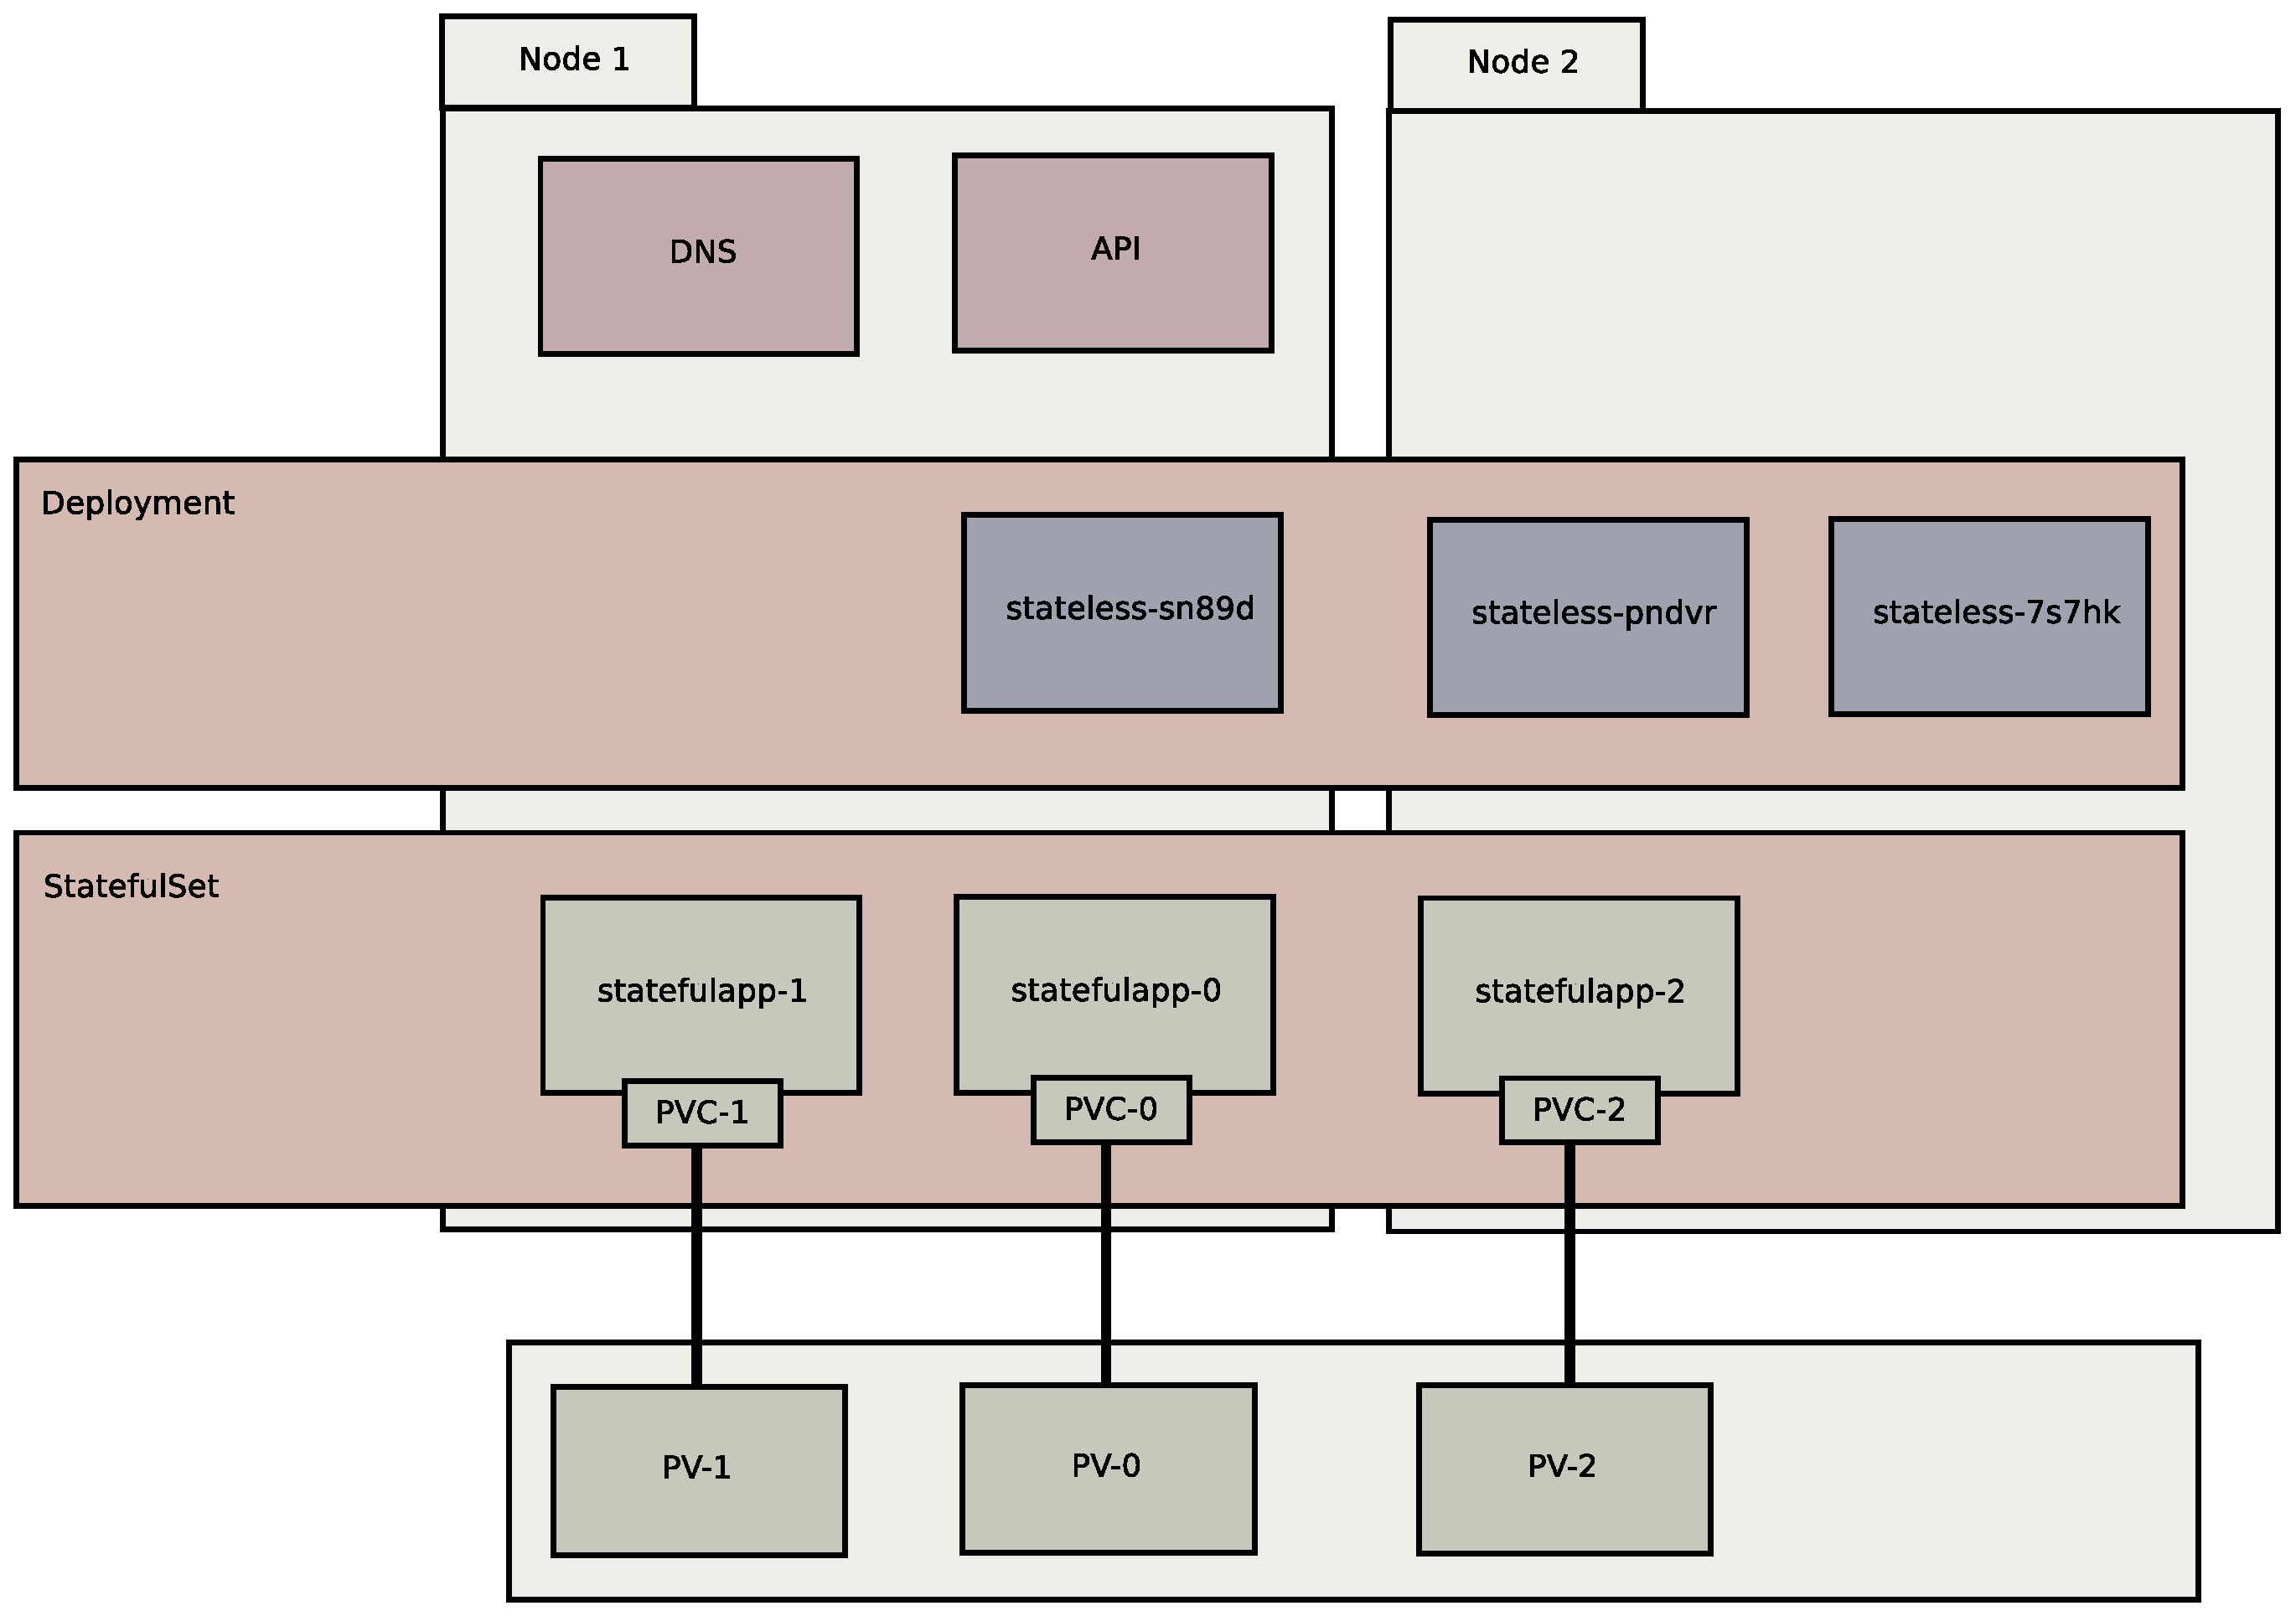
\includegraphics[width=\textwidth,height=0.85\textheight,keepaspectratio]{graphics/06-persistence.eps}
\end{frame}

\begin{frame}
    \frametitle{Headless Service}
    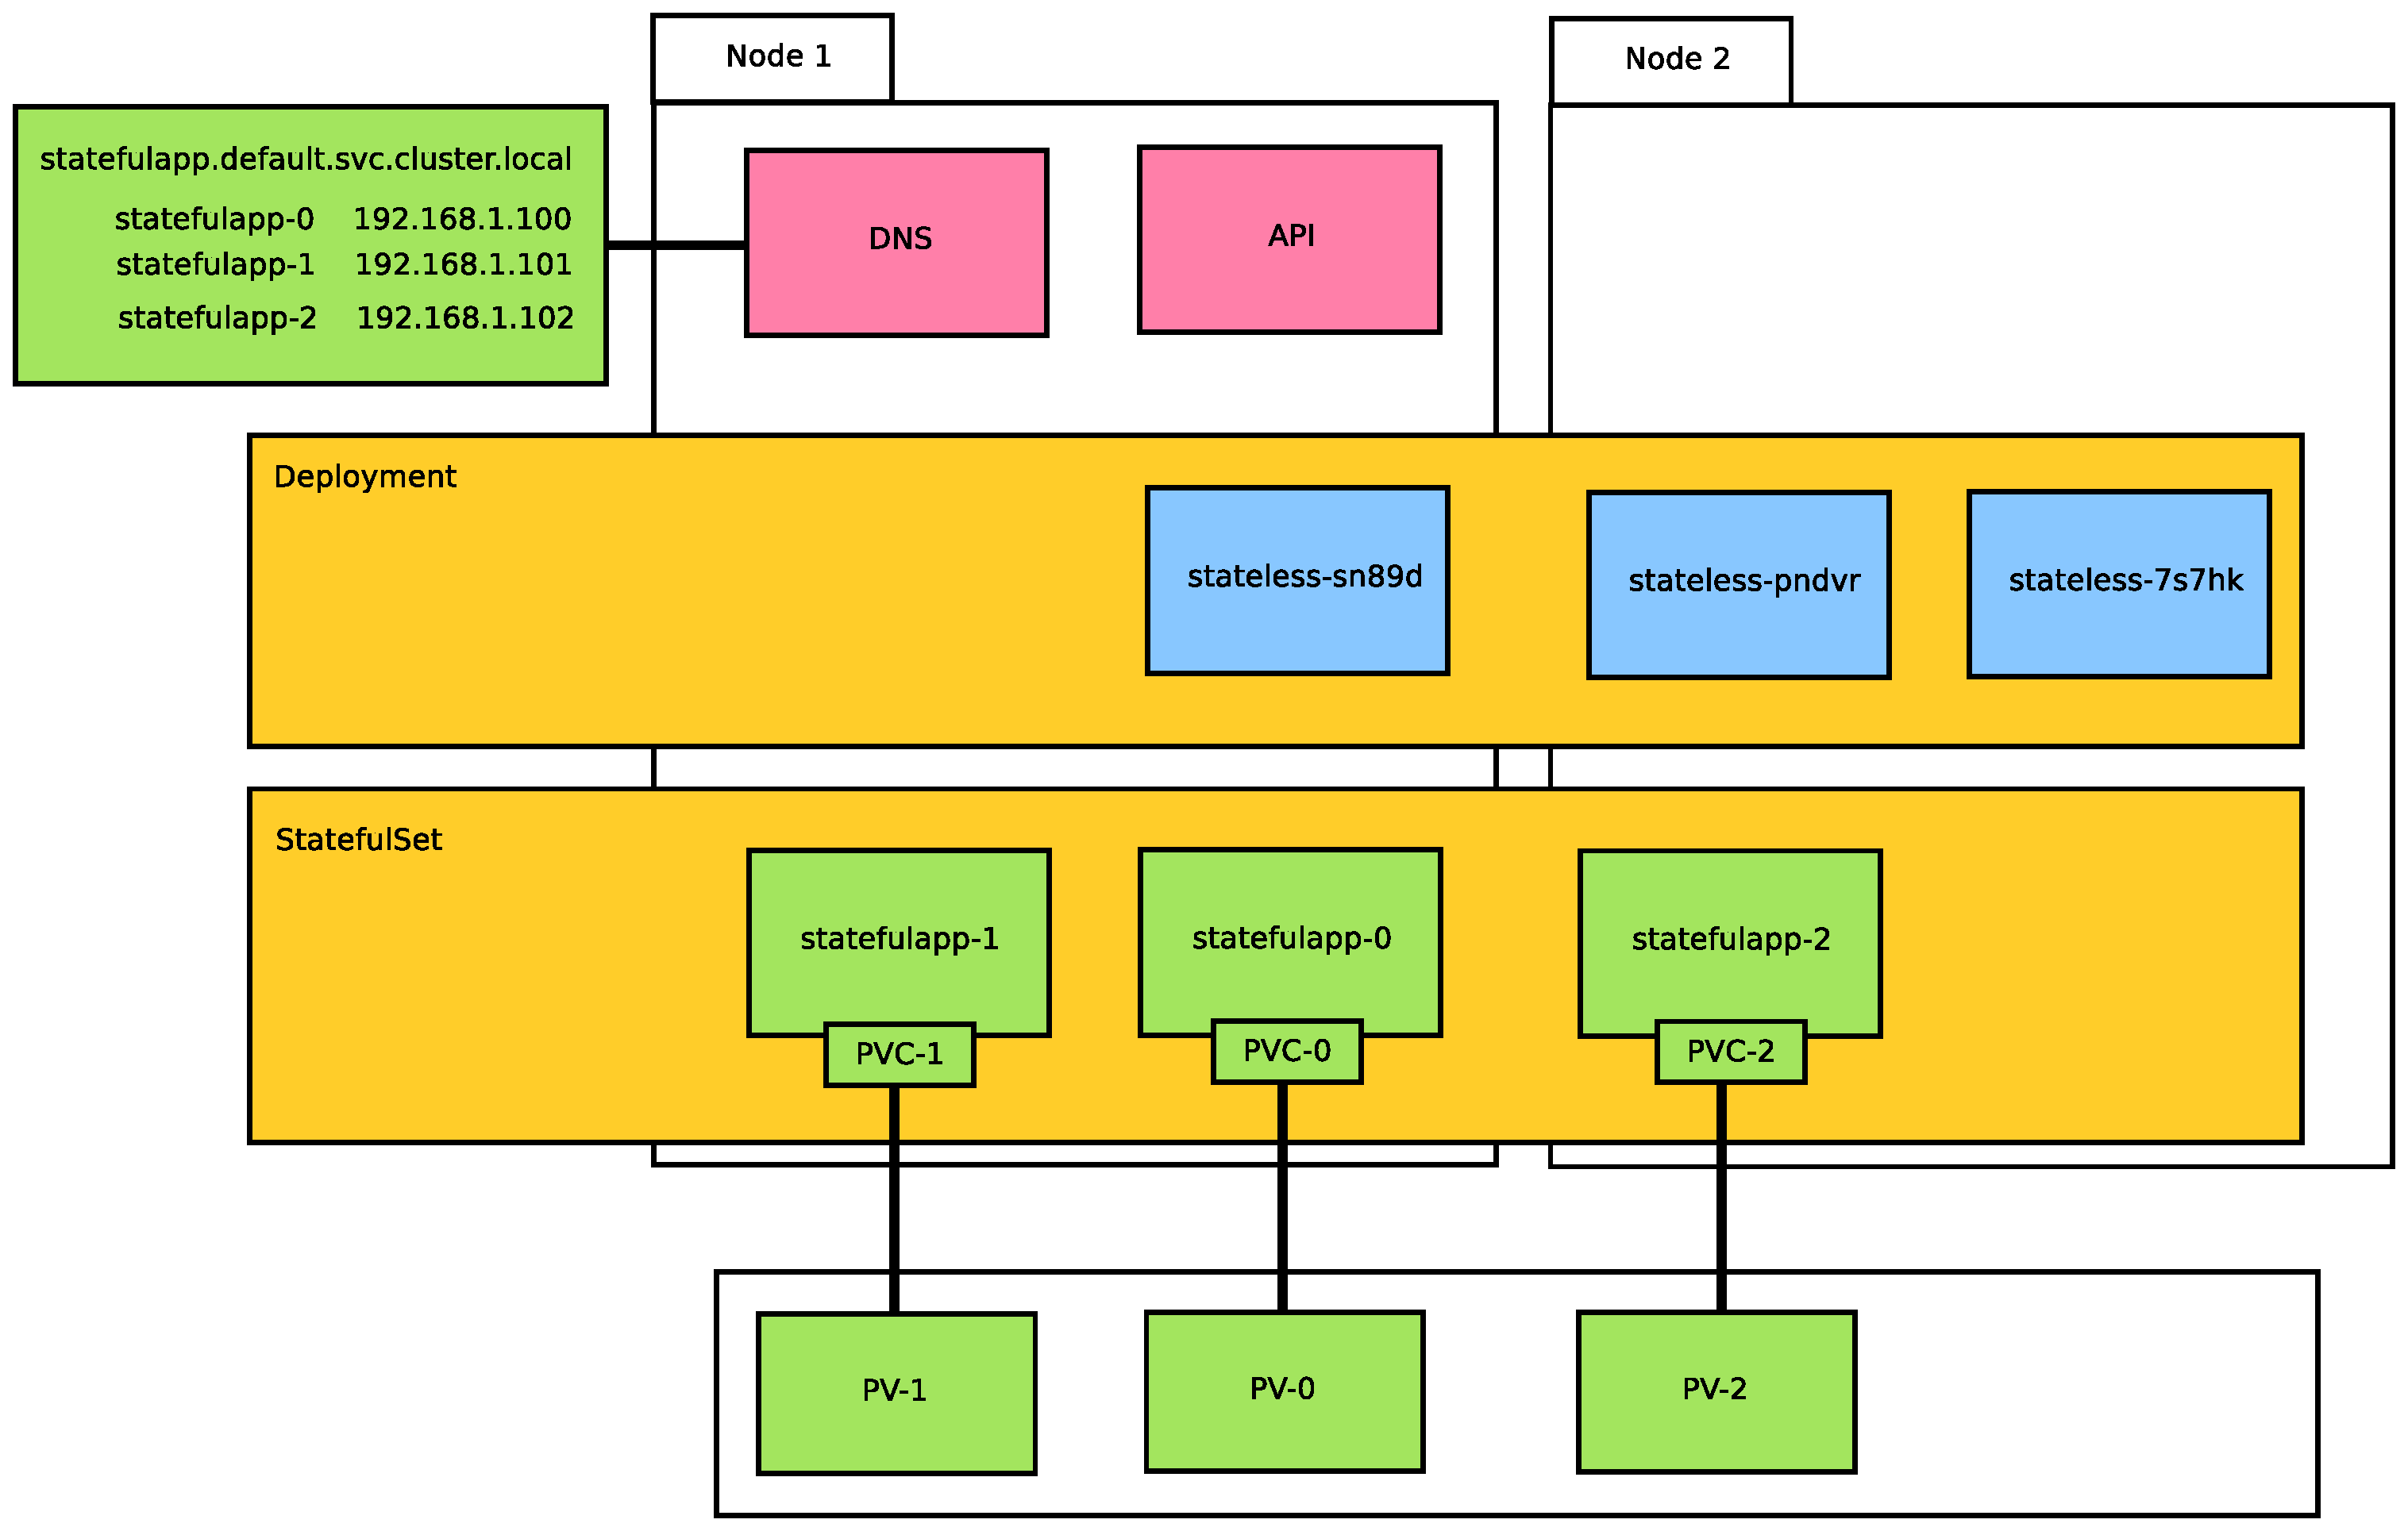
\includegraphics[width=\textwidth,height=0.85\textheight,keepaspectratio]{graphics/07-persistentIdentity.eps}
\end{frame}

\begin{frame}
    \frametitle{Load Balancers}
\end{frame}

\begin{frame}
    \frametitle{Load Balancing Services}
    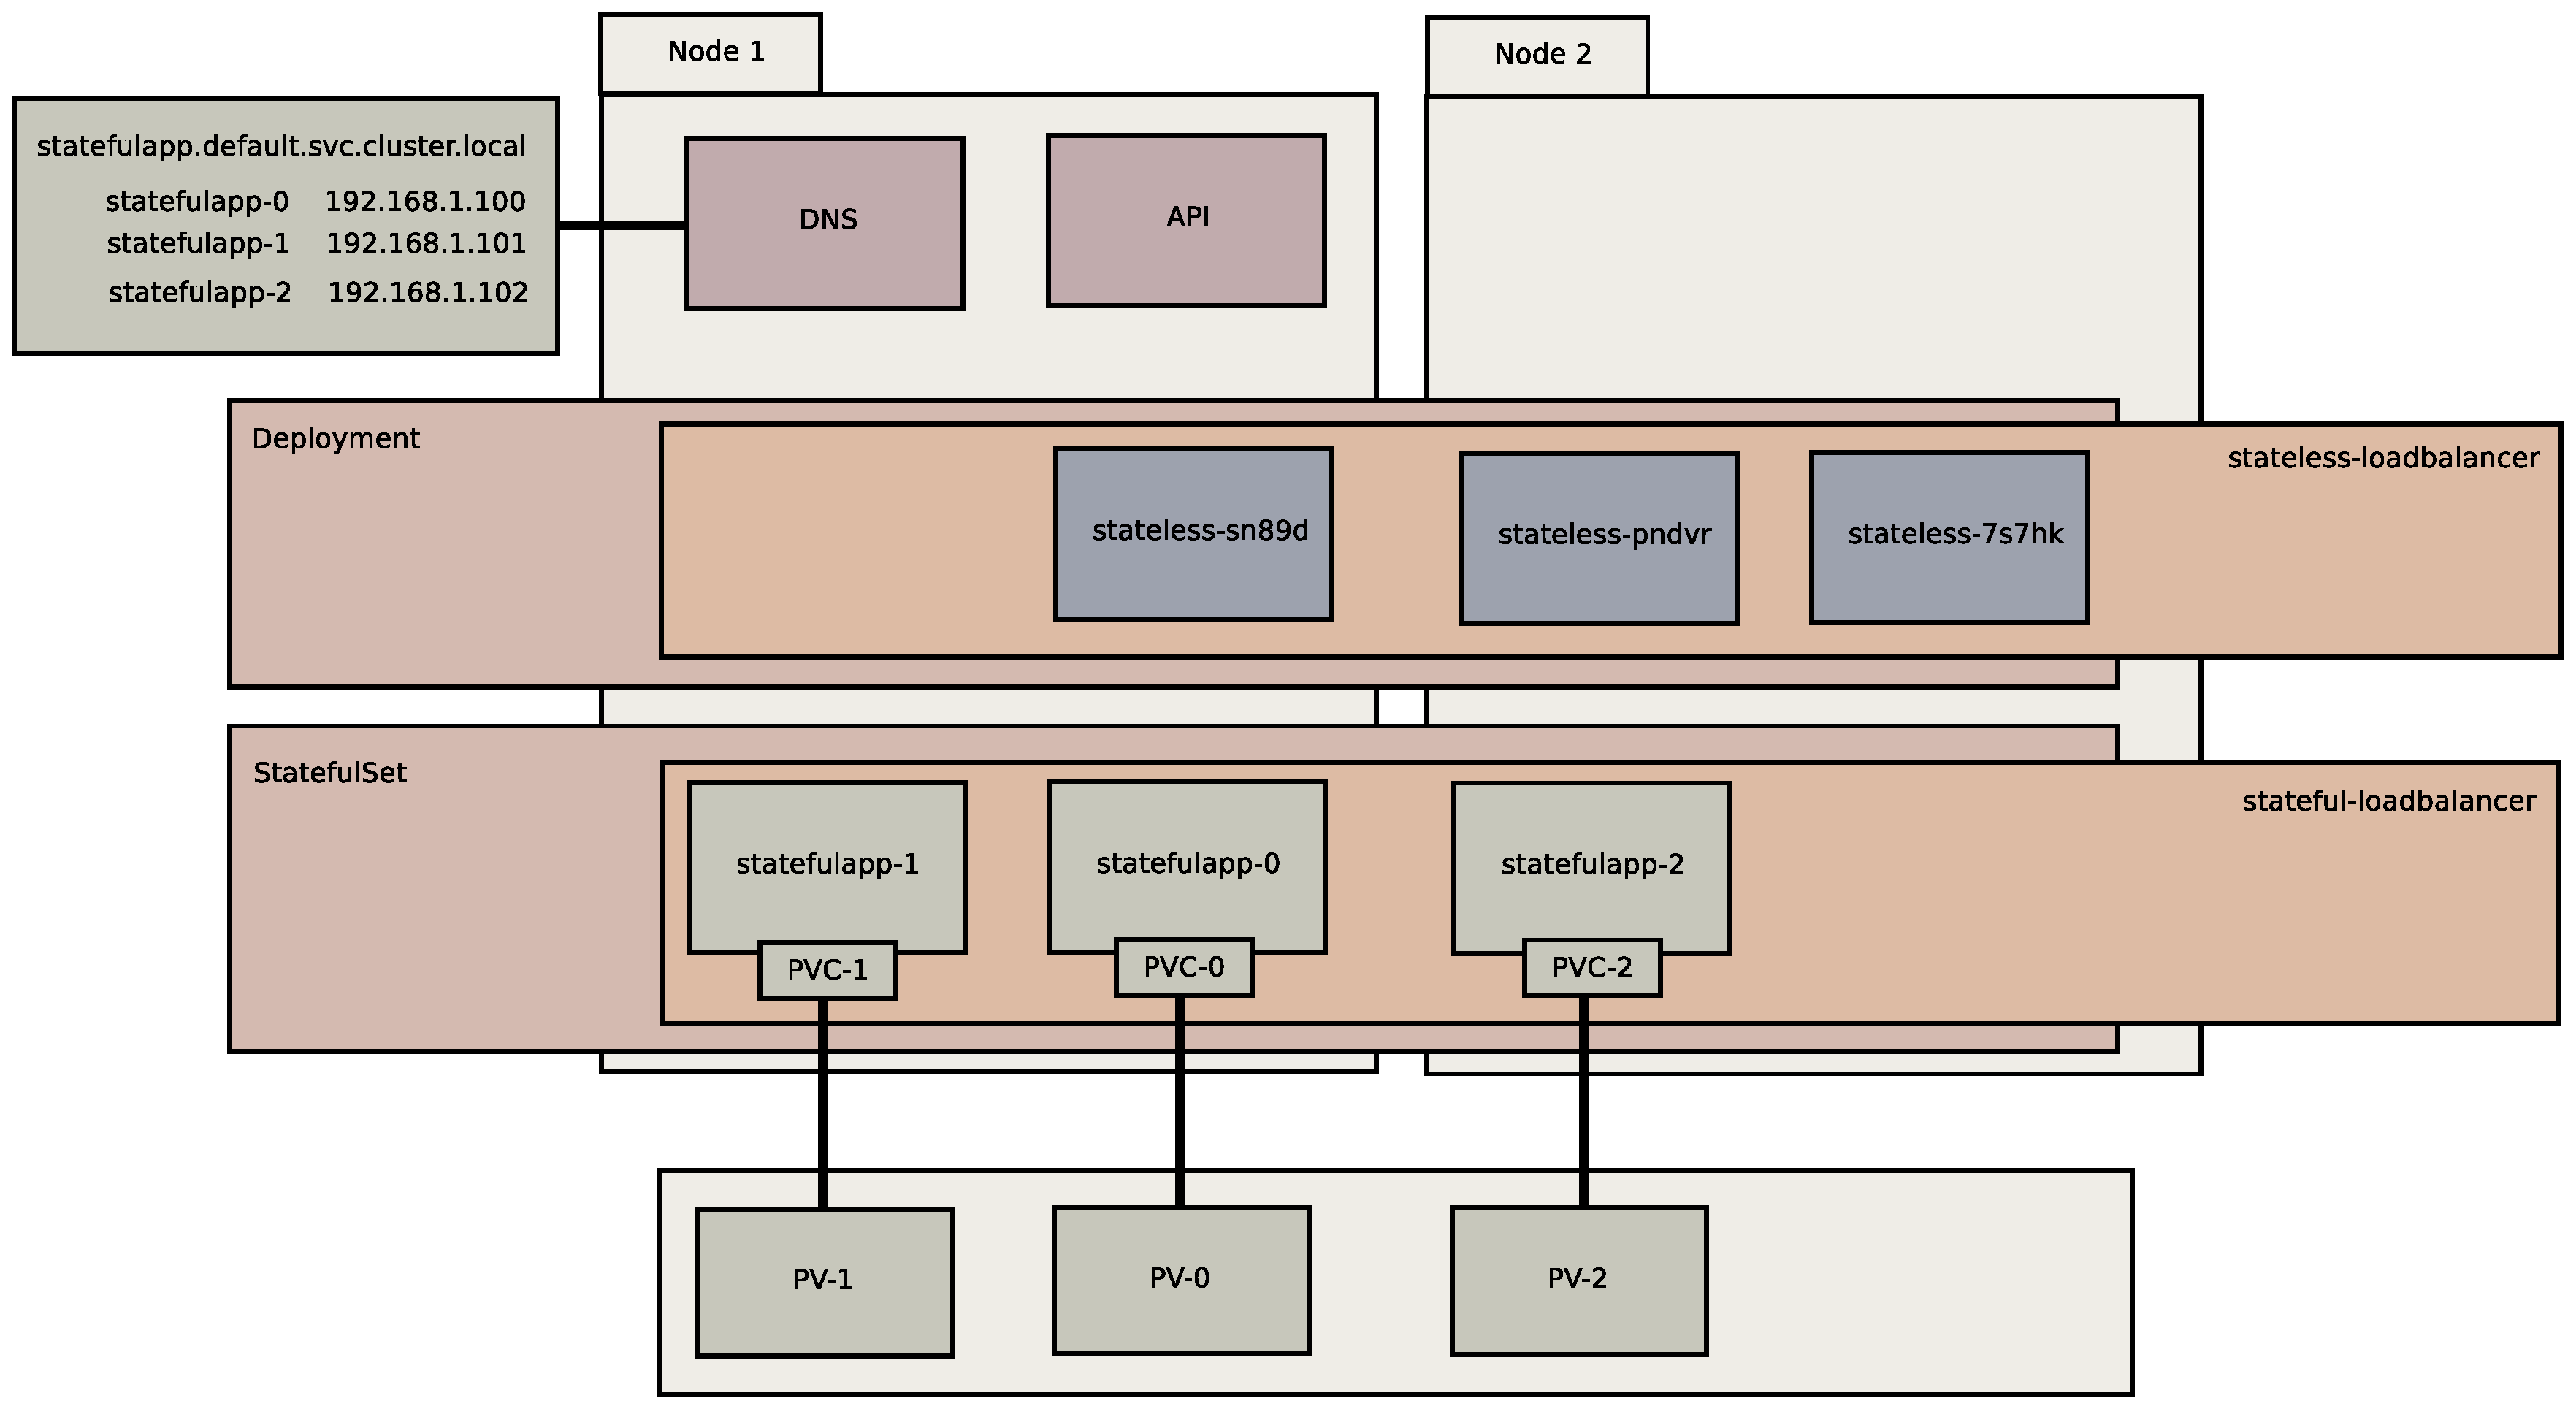
\includegraphics[width=\textwidth,height=0.85\textheight,keepaspectratio]{graphics/08-loadBalancer.eps}
\end{frame}

\begin{frame}
    \frametitle{Demo}
    \begin{center}
        \Huge So, let's see this in action!
    \end{center}
\end{frame}

\begin{frame}
    \frametitle{Overview}
    First, let's talk about the steps we're going to take:
    \begin{itemize}
        \item Start our Kubernetes environment (minikube).
        \item Configure our docker cli to talk to minikube's docker host.
        \item Build our two sample apps, package them as docker containers, and push the images.
        \item Run helm to deploy our applications.
        \item Proxy local ports to connect to our load balancing services.
    \end{itemize}
\end{frame}

\begin{frame}
    \frametitle{Demo}
    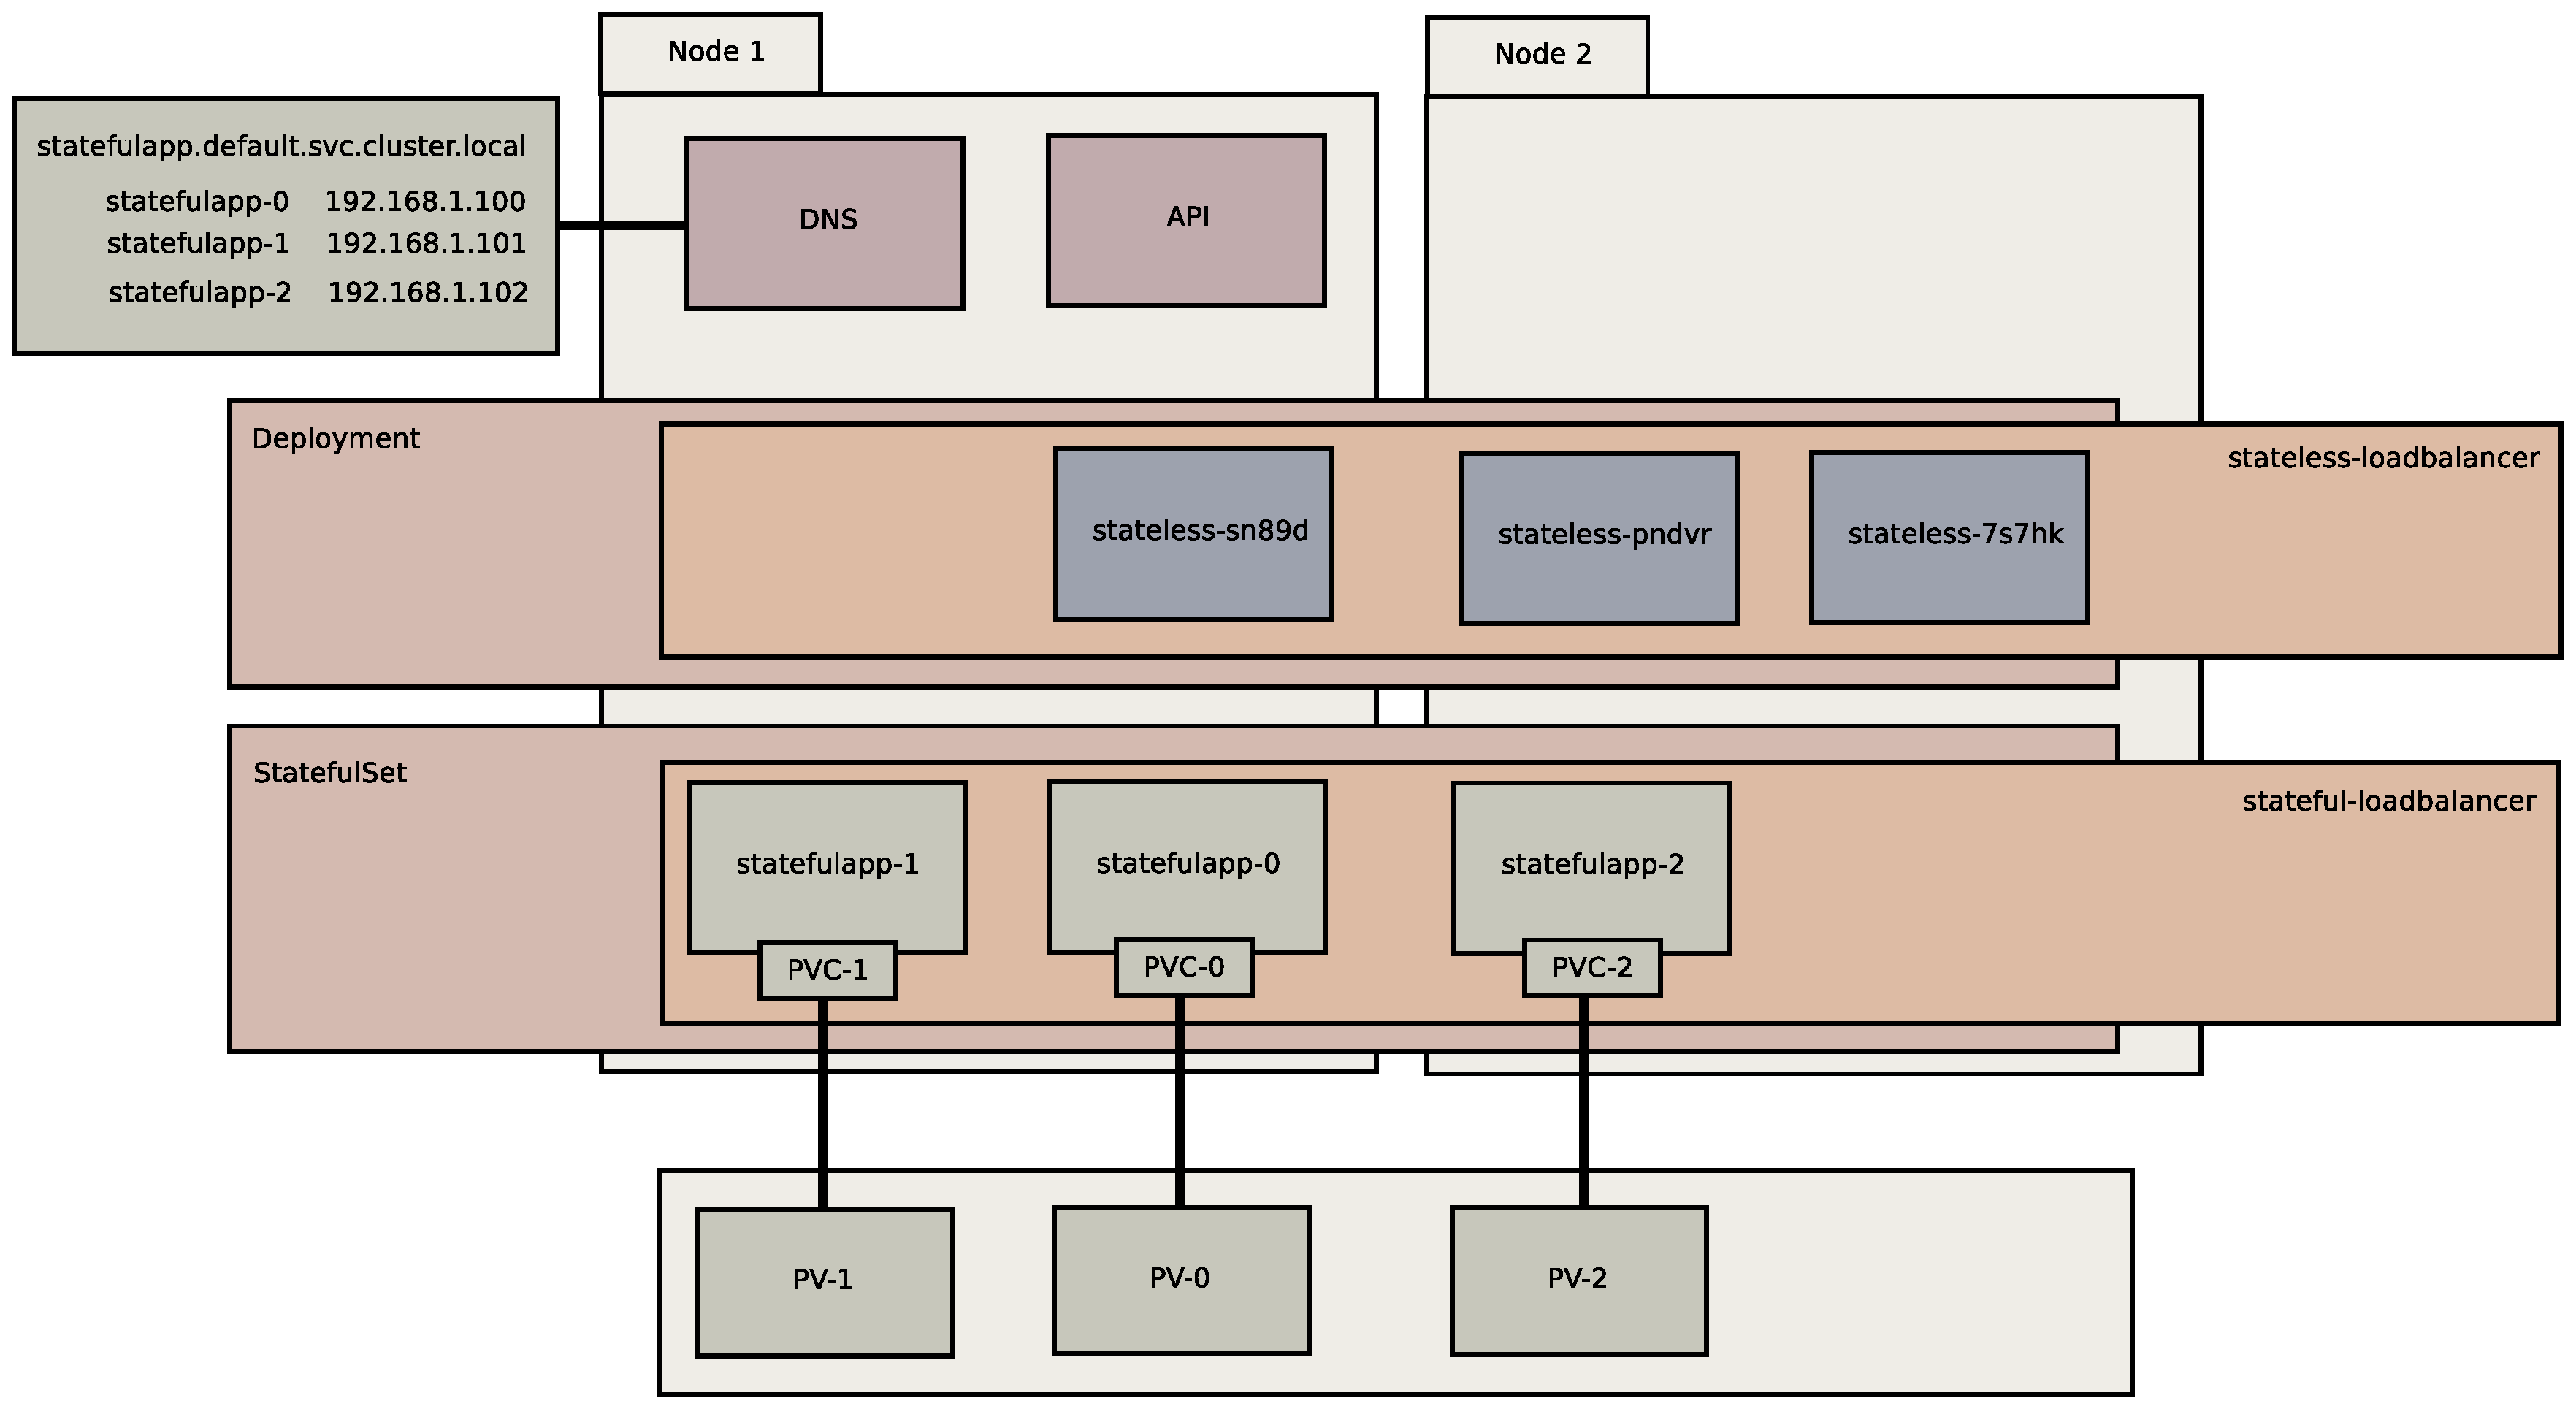
\includegraphics[width=\textwidth,height=0.85\textheight,keepaspectratio]{graphics/08-loadBalancer.eps}
\end{frame}

\begin{frame}
\frametitle{Other Resources}
Peripheral tools I used -- some of which warrant their own presentation
\begin{itemize}
    \item \LaTeX: \href{https://www.latex-project.org}{https://www.latex-project.org}
    \item Beamer: \href{https://ctan.org/pkg/beamer}{https://ctan.org/pkg/beamer}
    \item Kotlin: \href{https://kotlinlang.org}{https://kotlinlang.org}
    \item Spring Boot: \href{https://spring.io/projects/spring-boot}{https://spring.io/projects/spring-boot}
    \item Gradle: \href{https://gradle.org}{https://gradle.org}
    \item Dia: \href{http://dia-installer.de}{http://dia-installer.de}
\end{itemize}
\smallskip
Where I got my Subreddit data
\begin{itemize}
    \item Bulk Reddit data: \href{http://files.pushshift.io/reddit/subreddits}{http://files.pushshift.io/reddit/subreddits}
\end{itemize}
\end{frame}

\begin{frame}
    \begin{center}
        \Huge Questions?
    \end{center}
\end{frame}

%\begin{frame}
%\frametitle{What’s Still To Do?}
%\begin{block}{Answered Questions}
%    How many primes are there?
%\end{block}
%\begin{block}{Open Questions}
%    Is every even number the sum of two primes?
%\end{block}
%\end{frame}
%
%\begin{frame}
%\frametitle{What’s Still To Do?}
%\begin{columns}
%    \column{.25\textwidth}
%    \begin{block}{Answered Questions}
%        How many primes are there?
%    \end{block}
%    \column{.75\textwidth}
%    \begin{block}{Open Questions}
%        Is every even number the sum of two primes?
%    \end{block}
%\end{columns}
%\end{frame}
%
%\begin{frame}[fragile]
%\frametitle{An Algorithm For Finding Prime Numbers.}
%\begin{minted}{cpp}
%int main (void)
%{
%    std::vector<bool> is_prime (100, true);
%    for (int i = 2; i < 100; i++)
%        if (is_prime[i])
%        {
%            std::cout << i << " ";
%            for (int j = i; j < 100; is_prime [j] = false, j+=i);
%        }
%    return 0;
%}
%\end{minted}
%\end{frame}
%
%\begin{frame}[fragile]
%\frametitle{Yaml?}
%\begin{columns}
%    \column{.25\textwidth}
%    \begin{block}{Answered Questions}
%        How many primes are there?
%    \end{block}
%    \column{.75\textwidth}
%    \begin{block}{Open Questions}
%\begin{minted}[style=friendly,fontsize=\fontsize{3}{4}]{yaml}
%---
%apiVersion: v1
%kind: Pod
%metadata:
%  namespace: default
%  name: demo-demo-6f95ccf6d5-pdnmc
%  labels:
%    app.kubernetes.io/instance: demo
%    app.kubernetes.io/name: demo
%spec:
%  containers:
%  - image: nginx:1.16.0
%    name: demo
%    livenessProbe:
%      httpGet:
%        path: /
%        port: http
%        scheme: HTTP
%    ports:
%    - containerPort: 80
%      name: http
%      protocol: TCP
%    readinessProbe:
%      httpGet:
%        path: /
%        port: http
%        scheme: HTTP
%    volumeMounts:
%    - mountPath: /var/run/secrets/kubernetes.io/serviceaccount
%      name: demo-demo-token-dj7lr
%      readOnly: true
%  volumes:
%  - name: demo-demo-token-dj7lr
%    secret:
%      defaultMode: 420
%      secretName: demo-demo-token-dj7lr
%
%\end{minted}
%    \end{block}
%\end{columns}
%\end{frame}

\end{document}
